\documentclass[]{memoir}
\title{Problem Set 4}
\author{Brian Fox}
\date{}
\usepackage{enumitem}
\usepackage{geometry}
\geometry{margin=30mm}
\usepackage{graphicx}
\usepackage{multicol}
\usepackage{amsmath}
\begin{document}
\maketitle

\begin{enumerate}

\item \textit{25.2-1} Run the Floyd-Warshall algorithm on the weighted, directed graph of Figure 25.2. Show the matrix $D^{(k)}$ that results for each iteration of the outer loop.
\paragraph{} fig 25.2:
\begin{figure}[h]
	\centering
	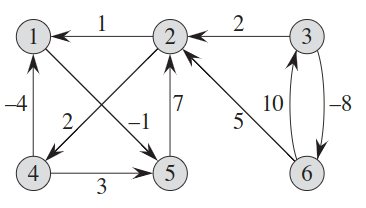
\includegraphics[scale=.5]{25-2}
\end{figure}

\begin{align*}
D^{(0)} & \begin{bmatrix}
	0 & \infty & \infty & \infty & -1 & \infty \\
	1 & 0 & \infty & 2 & \infty & \infty \\
	\infty & 2 & 0 & \infty & \infty & -8 \\
	-4 & \infty & \infty & 0 & 3 & \infty  \\
	\infty & 7 & \infty & \infty & 0 & \infty \\
	\infty & 5 & 10 & \infty & \infty & 0 \\ 
\end{bmatrix}
&
D^{(3)} & \begin{bmatrix}
	0 & \infty & \infty & \infty & -1 & \infty \\
	1 & 0 & \infty & 2 & 0 & \infty \\
	3 & 2 & 0 & 4 & 2 & -8 \\
	-4 & \infty & \infty & 0 & -5 & \infty  \\
	8 & 7 & \infty & 9 & 0 & \infty \\
	6 & 5 & 10 & 7 & 5 & 0 \\ 
\end{bmatrix}
\end{align*}
\begin{align*}
D^{(1)} & \begin{bmatrix}
	0 & \infty & \infty & \infty & -1 & \infty \\
	1 & 0 & \infty & 2 & 0 & \infty \\
	\infty & 2 & 0 & \infty & \infty & -8 \\
	-4 & \infty & \infty & 0 & -5 & \infty  \\
	\infty & 7 & \infty & \infty & 0 & \infty \\
	\infty & 5 & 10 & \infty & \infty & 0 \\ 
\end{bmatrix}
&
D^{(4)} & \begin{bmatrix}
	0 & \infty & \infty & \infty & -1 & \infty \\
	-2 & 0 & \infty & 2 & -3 & \infty \\
	0 & 2 & 0 & 4 & -1 & -8 \\
	-4 & \infty & \infty & 0 & -5 & \infty  \\
	5 & 7 & \infty & 9 & 0 & \infty \\
	3 & 5 & 10 & 7 & 2 & 0 \\ 
\end{bmatrix}
\end{align*}
\begin{align*}
D^{(2)} & \begin{bmatrix}
	0 & \infty & \infty & \infty & -1 & \infty \\
	1 & 0 & \infty & 2 & 0 & \infty \\
	3 & 2 & 0 & 4 & 2 & -8 \\
	-4 & \infty & \infty & 0 & -5 & \infty  \\
	8 & 7 & \infty & 9 & 0 & \infty \\
	6 & 5 & 10 & 7 & 5 & 0 \\ 
\end{bmatrix}
&
D^{(5)} & \begin{bmatrix}
	0 & 6 & \infty & 8 & -1 & \infty \\
	-2 & 0 & \infty & 2 & -3 & \infty \\
	0 & 2 & 0 & 4 & -1 & -8 \\
	-4 & 2 & \infty & 0 & -5 & \infty  \\
	5 & 7 & \infty & 9 & 0 & \infty \\
	3 & 5 & 10 & 7 & 2 & 0 \\ 
\end{bmatrix}
\end{align*}
\begin{align*}
D^{(6)} & \begin{bmatrix}
	0 & 6 & \infty & 8 & -1 & \infty \\
	-2 & 0 & \infty & 2 & -3 & \infty \\
	-5 & -3 & 0 & -1 & -6 & -8 \\
	-4 & 2 & \infty & 0 & -5 & \infty  \\
	5 & 7 & \infty & 9 & 0 & \infty \\
	3 & 5 & 10 & 7 & 2 & 0 \\ 
\end{bmatrix}
\end{align*}

\item \textit{27.1-5} Professor Karan measures her  deterministic multithreaded  algorithm  on 4, 10, and 64 processors  of  an  ideal  parallel  computer  using  a  greedy  scheduler.   She claims  that  the  three  runs  yielded T=4 D=80 seconds, T=10 D=42 seconds,  and T=64 D=10 seconds.  Argue that the professor is either lying or incompetent.  (Hint:Use the  work law (27.2),  the  span  law (27.3),  and  inequality  (27.5)  from  Exercise 27.1-3.)

\item \textit{27.1-7} Consider the following multithreaded pseudocode for transposing an $n\times n$ matrix A in place:\\
P-TRANSPOSE(A)
\begin{enumerate}[label=\arabic*\hspace{2mm}]
	\item $n = A.rows$	
	\item \textbf{parallel for} j=2 \textbf{to} n
	\item \hspace{1cm} \textbf{parallel for} i=1 \textbf{to} j-1
	\item \hspace{2cm} exchange $a_{ij}$ with $a_{ji}$
\end{enumerate}
Analyze the work, span, and parallelism of this algorithm.
\paragraph{}
\begin{Large}
The work, $T_{1}=\Theta{}(n^{2})$. The span, $T_{\infty} = \Theta{}(\lg{n})$. Therefor the parallelism of the algorithm is $\Theta{}(\frac{n^{2}}{\lg{n}})$.
\end{Large}
\\\item \textit{27.1-8} Suppose that we replace the parallel for loop in line 3 of P-TRANSPOSE (see Exercise 27.1-7) with an ordinary for loop.  Analyze the work, span, and parallelism of the resulting algorithm.
\paragraph{}
\begin{Large}
The work, $T_{1}=\Theta{}(n^{2})$. The span, $T_{\infty} = \Theta{}(n)$. Therefor the parallelism of the algorithm is $\Theta{}(n)$.
\end{Large}
\\\item \textit{27.2-6} Give 
pseudocode for an efficient multithreaded implementation of the Floyd-Warshall algorithm (see Section 25.2), which computes shortest paths between all pairs of vertices in an edge-weighted graph. Analyze your algorithm.

FLOYD-WARSHALL(W)
\begin{enumerate}[label=\arabic*\hspace{2mm}]
	\item $n = W.rows$	
	\item $D^{(0)} = W$
	\item \textbf{for} $k=1$ \textbf{to} $n$
	\item \hspace{1cm} let $D^{(k)}=\left( d_{ij}^{(k)}\right)$ be a new $n \times n$ matrix
	\item \hspace{1cm} \textbf{parallel for} $i=1$ \textbf{to} n
	\item \hspace{2cm} \textbf{parallel for} $j=1$ \textbf{to} n
	\item \hspace{3cm} $d_{ij}^{(k)}= \min{(d_{ij}^{(k-1)},d_{ik}^{(k-1)} + d_{kj}^{(k-1)})}$
	\item \textbf{return} $D^{(n)}$
\end{enumerate}
\paragraph{}
\begin{Large}
The work, $T_{1}=\Theta{}(n^{3})$. The span, $T_{\infty} = \Theta{}(n\lg{n})$. Therefor the parallelism of the algorithm is $\Theta{}(\frac{n^{2}}{\lg{n}})$.
\end{Large}
\\\item \textit{27-1}, all 3 parts: part a is on page 805, parts b and c are on page 806.
\begin{enumerate}
\item 
SUM-ARRAYS($A,B,C,i,i'$)
\begin{enumerate}[label=\arabic*\hspace{2mm}]
	\item \textbf{if} $i == i'$
	\item \hspace{1cm} $C[i] = A[i] + B[i]$
	\item \textbf{else} $mid = \lfloor (i+i')/2 \rfloor$
	\item \hspace{1cm} \textbf{spawn} SUM-ARRAYS($A,B,C,i,mid$)
	\item \hspace{1cm} SUM-ARRAYS($A,B,C,mid+1,i'$)
	\item \hspace{1cm} \textbf{sync}
\end{enumerate}
\item
For grain size one the parallelism of the equation is constant because there is no improvement over a serial for loop.
\item
$$T_{\infty} = \Theta{}(\frac{r}{n}+r)$$
The optimal value for r is $\sqrt{n}$. I don't know how to determine this so I just asked wolfram alpha to minimize with respect to r and provided a few random constants for n. For whatever value of n I gave the calculator returned $\sqrt{n}$.
\end{enumerate}
\item Design a parallel version of the naive-string-matcher algorithm from page 988 of the book.  Describe your algorithm with pseudocode.
        Compute the work, T subscript 1 , of your parallel naive string matcher.
        Compute the span, T subscript infinity , of your parallel naive string matcher.
        Compute the parallelism, bevelled T subscript 1 over T subscript infinity , of your parallel naive string matcher.
        Compute the runtime on P processors, T subscript P , of your parallel naive string matcher.

NAIVE-STRING-MATCHER($T,P$)
\begin{enumerate}[label=\arabic*\hspace{2mm}]
	\item $n = T.length$
	\item $m = P.length$
	\item \textbf{for} $s = 0$ \textbf{to} $n-m$
	\item \hspace{1cm} if $P[1] == T[s+1]$
	\item \hspace{2cm} \textbf{spawn} PARALLEL-MATCHER($T,P,s$) 
\end{enumerate}
PARALLEL-MATCHER($T,P$)
\begin{enumerate}[label=\arabic*\hspace{2mm}]
	\item $m = P.length$
	\item \textbf{if} $P[1...m] == T[s+1...s+m]$
	\item \hspace{1cm} print "Pattern occurs with shift" s
\end{enumerate}
\paragraph{}
\begin{Large}
$T_{1} = \Theta{}(nm)$.
$T_{\infty} = \Theta{}(n)$ since we can continue to iterate over $T$ as we check if a match occurs at a given shift $s$.
$T_{P} = \Theta{}(n)$ since there will always be one thread that has to iterate over each index of $T$.
\end{Large}
\end{enumerate}
\end{document}

